% !TEX root = exercises_1.tex
% !TeX encoding = UTF-8
% !TeX spellcheck = en_US
\documentclass[a4paper]{scrartcl}
\usepackage[T1]{fontenc}
%\usepackage[utf8]{inputenc}
\usepackage[english]{babel}
\usepackage[bottom=2.5cm,top=2.0cm,left=2.0cm,right=2.0cm]{geometry}
\usepackage{amssymb,amsmath,amsfonts}
\usepackage{lmodern}
\usepackage{csquotes}
\usepackage{url}
\usepackage{doi}
\usepackage{hyperref}
\usepackage{enumitem}
\usepackage{graphicx}
\usepackage[dvipsnames]{xcolor}
\definecolor{mygreen}{rgb}{0,0.4,0}
\definecolor{mygray}{rgb}{0.5,0.5,0.5}
\usepackage[numbered,framed]{matlab-prettifier}
\usepackage[backend=biber,style=authoryear]{biblatex}
\addbibresource{literature/_biblio.bib}
\usepackage[stable]{footmisc}
\usepackage{booktabs,longtable}
\usepackage{nameref}
\usepackage{float}
\usepackage{tikz}
\usetikzlibrary{positioning}
\usetikzlibrary{decorations.text}
\renewcommand{\contentsname}{Overview}

\usepackage[
	%nosolutionfiles
	]{answers}

\Newassociation{solution}{Solution}{exercises_1_solution}
\newif\ifDisplaySolutions\DisplaySolutionstrue%

\begin{document}
\title{Computational Macroeconomics\\~\\Summer 2025\\~\\Exercise Sheet 1}
\author{Willi Mutschler\\willi@mutschler.eu}
\date{Version: 1.0\\Latest version available on: \href{https://github.com/wmutschl/Computational-Macroeconomics/releases/latest/download/exercises_1.pdf}{GitHub}}
\maketitle\thispagestyle{empty}

\newpage
\Opensolutionfile{exercises_1_solution}[exercises_1_solution]
\tableofcontents\thispagestyle{empty}\newpage

\setcounter{page}{1}
\section[What is Computational Macroeconomics]{What is Computational Macroeconomics\label{ex:ComputationalMacroeconomics}}
Broadly define the scope and research topics of \enquote{Computational Macroeconomics}, 
	  sometimes referred to as \enquote{Numerical Methods in Macroeconomics}.
What are the challenges and approaches?

\paragraph{Readings}
\begin{itemize}
	\item \textcite[Ch. 1-2]{Fernandez-Villaverde.Rubio-Ramirez.Schorfheide_2016_SolutionEstimationMethods}
	\item \textcite[Ch. 1-2]{Maliar.Maliar_2014_NumericalMethodsLargeScale}
	\item \textcite[Ch. 1]{Judd_1998_NumericalMethodsEconomics}
\end{itemize}

\begin{solution}\textbf{Solution to \nameref{ex:ComputationalMacroeconomics}}
\ifDisplaySolutions
\input{exercises/computational_macroeconomics_scope_solution.tex}
\fi
\newpage
\end{solution}\newpage
\section[Programming Languages]{Programming Languages\label{ex:ProgrammingLanguages}}
\begin{enumerate}
\item Name some popular programming languages in macroeconomics.
Which are general purpose, which are domain specific?
\item What are the differences between compiled and interpreted languages?
\item What is important when choosing a programming language for scientific computing in macroeconomics?
Which programming language{(s)} would you choose?
\end{enumerate}

\paragraph{Readings}
\begin{itemize}
\item \textcite{Aguirre.Danielsson_2020_WhichProgrammingLanguage}
\item \textcite{Aruoba.Fernandez-Villaverde_2015_ComparisonProgrammingLanguages} (note the Update available at \url{https://www.sas.upenn.edu/~jesusfv/Update_March_23_2018.pdf})
\end{itemize}

\begin{solution}\textbf{Solution to \nameref{ex:ProgrammingLanguages}}
\ifDisplaySolutions%
\begin{enumerate}
\item General purpose: C/C++, Fortran, Python, Excel.
	Domain-specific: MATLAB, Julia, R, Mathematica, EViews.
\item Every program is a set of instructions, say to add two numbers. 
	Compilers and interpreters take human-readable code and convert it to computer-readable machine code.
	In a compiled language, the target machine directly translates the program.
	In an interpreted language, the source code is not directly translated by the target machine.
	Instead, a different program, aka the interpreter, reads and executes the code.
	Some modern languages like Python can have both compiled and interpreted implementations,
	  but for simplicity's sake it is useful to keep in mind the distinction.
		
	Compiled languages like Fortran, C or C++ are usually fastest, more efficient and more powerful,
	  but they are harder to learn and harder to code in.
	They also require a build step, i.e. they need to be compiled.
	Interpreted languages like Python, Mathematica, MATLAB, R or Julia are slower,
	  but easier to learn and faster to code in.
	Interpreters run through a program line by line and execute each command.
	Interpreted languages tend to be very similar in the syntax,
	  but differ in best practices and concepts.
	
	Interpreted languages were once significantly slower than compiled languages.
	But, with the development of just-in-time (JiT) compilation, that gap is shrinking.
	MATLAB and Julia are two very prominent examples that make use of JiT compilation,
	  that is they combine both worlds.

	You can also make use of e.g. Fortran or C++ code in MATLAB, R, Python or Julia;
	  that is, write very CPU-intensive tasks in a compiled language
	  and use them in an interpreted language.
	
\item Learning a programming language is a huge investment;
	however, once one has knowledge of one, learning another one tends to be easier
	  as they are based on similar principles.
	Try to stick with popular choices as the choice of learning resources and communities
	  that help you learn this language are wider spread,
	  i.e. googling for help is much easier for C++ than for Fortran.
	Often the project you are working on dictates which programming language you should use.
	The general purpose languages can be used in many non-scientific applications,
	  so your investment might payoff in very different fields in the end. 
		
	In scientific computing, particularly in Macroeconomics,
	  we are often faced with CPU intensive problems 
	  and need to prototype models and methods quickly.
	An interpreted language like MATLAB or Julia that does just-in-time compilation
	  is therefore best suited for such tasks.
	Moreover, having some basic knowledge in C++ is advisable
	  to write computational intensive tasks in a compiled language 
	  and reuse this as e.g. so-called MEX files in MATLAB.
	Moreover, looking at legacy code in the last 20-30 years of research done
	  in quantitative and computational Macroeconomics,
	  we see that most was and still is conducted in MATLAB,
	  whereas highly intensive tasks were programmed in Fortran.
	So keep in mind, that you need to understand this legacy codebase.
	Nevertheless, in the last couple of years, researchers in Macroeconomics are really pushing Julia.
	Moreover, new developments like Machine Learning require you to invest in Python.
	For writing scientific reports and papers you should get familiar with Latex and Markdown.
	
	Another issue to consider is the license, cost and support of the language maintainers.
	Most programming languages are free and open-source,
	  others like MATLAB are proprietary and are quite expensive
	  (luckily there are free and open-source clones like Octave available).
	Regardless of the license, having a good governance structure,
	  i.e. a board, cooperation or company driving the development of the language,
	  is very important for the sustainability of the language
	  and for your investment in a computer language.
			
	Lastly, and very importantly, have a look at the toolset available for the languages.
	Which Integrated Development Environment (IDE) do you like best?
	Which text editor do you prefer?
	How good are the debugging capabilities of your chosen environment.
	Things like syntax highlighting, smart indentation, code linting, comparison tools,
	  handling of workspace, etc. are very important.
	Some languages like MATLAB bring their own IDE in one big package and it works very well.
	Others like Julia, Python or C++ can be neatly integrated in a variety of environments;
	  in fact Visual Studio Code has become the leading editor and environment for many languages,
	  but of course there are many other great choices depending on your needs and preferences.
	
	So which computer languages should you devote your time into,
	  if you are interested in computational or quantitative macroeconomics?
	\\
	\textbf{Here is my opinionated advice:}
	\begin{itemize}
		\item Default languages (excellent knowledge): Julia and MATLAB
		\item Data analysis and Machine Learning (advanced knowledge): R and Python
		\item Heavy tasks (basic knowledge): C++ and Fortran
		\item Scientific writing (advanced knowledge): Markdown and Latex
	\end{itemize}
\end{enumerate}
\fi
\newpage
\end{solution}\newpage
\input{exercises/matlab_quick_tour.tex}\newpage
\section[ARMA{(1,1)} Simulation]{ARMA{(1,1)} Simulation\label{ex:ARMASimulation}}
Consider the ARMA{(1,1)} model:
\begin{align*}
x_t - \theta x_{t-1} = \varepsilon_t - \phi \varepsilon_{t-1}
\end{align*}
where \(\varepsilon_t \sim N(0,1)\).

\begin{enumerate}

\item
Compute the non-stochastic steady-state with pen and paper,
  i.e.\ what is the value of \(x_t\) if \(\varepsilon_t = 0\) for all \(t\)?

\item
Write a Dynare mod file for this model:

\begin{itemize}

\item
\(x\) is the endogenous variable, \({\varepsilon}\) the exogenous variable, and \({\theta}\) and \({\phi}\) are the parameters.

\item
Set \(\theta = \phi = 0.4\).

\item
Write either a \texttt{steady\_state\_model} or \texttt{initval} block and compute the steady-state.

\item
Start at the non-stochastic steady-state and simulate 200 data points using a \texttt{shocks} block
  and the \texttt{stoch\_simul} command.
Plot both \(x\) as well as \({\varepsilon}\) using \texttt{rplot}.

\item
Try out different values for \({\theta}\) and \({\phi}\).
What do you notice?

\end{itemize}

\item
Redo the exercise in MATLAB without using Dynare.

\end{enumerate}

\emph{Hints}:

\begin{itemize}

\item
Don't forget to add Dynare's matlab folder:
\texttt{addpath C:/dynare/6.0/matlab} for Windows,
\texttt{addpath /Applications/Dynare/6.0/matlab} for macOS,
\texttt{addpath /opt/dynare/6.0/matlab} for Linux machines.
If you installed Dynare to a different folder, adapt the path accordingly.

\item
When saving your Dynare script as a mod file, try to use a simple name.
That is, don't use special characters or spaces in the filename, e.g.\
  \texttt{arma{(1,1)}.mod} as well as \texttt{arma 1 1.mod} are not valid filenames,
  whereas \texttt{arma.mod} or \texttt{arma\_1\_1.mod} or \texttt{arma11.mod} are valid.

\item
It is advised to save the mod file directly on your hard drive and not on a cloud storage drive.
If you do save it to a folder that is in sync with e.g.\ Dropbox, iCloud, Nextcloud, OneDrive (etc),
  please (temporarily) deactivate sync activities,
  to prevent sync conflicts and weird errors when running Dynare.

\end{itemize}


\begin{solution}\textbf{Solution to \nameref{ex:ARMASimulation}}
\ifDisplaySolutions%
\begin{enumerate}

\item
As for all \(t\) the shocks are zero, i.e.\
  \(\varepsilon_t = 0\), we get \(x - \theta x = 0 \Leftrightarrow x = 0\),
  where \(x\) denotes the non-stochastic steady-state
  (we drop the time subscript in the original equation when computing the steady-state).

\item
\lstinputlisting[style=Matlab-editor,basicstyle=\mlttfamily\scriptsize,title=\lstname]{progs/dynare/arma11.mod}

Some notes:

\begin{itemize}

\item
Whenever the parameters are equal to each other, the simulated series for \(x_t\) is always equal to the drawn shocks \(\varepsilon_t\).

\item
Sometimes Dynare prints an error message, e.g.\ try out \(\theta=1.5\) and \(\theta=0.4\).
If you are familiar with time series models, this is due to the fact that this parameter combination provides a non-stationary process,
  i.e.\ the process explodes and does not return to the equilibrium/steady-state.
\end{itemize}

\item
This function simulates the ARMA{(1,1)} model in MATLAB:\@
\lstinputlisting[style=Matlab-editor,basicstyle=\mlttfamily\scriptsize,title=\lstname]{progs/matlab/arma11Simulate.m}
This script can be used to compare the results from Dynare with the results from MATLAB:\@
\lstinputlisting[style=Matlab-editor,basicstyle=\mlttfamily\scriptsize,title=\lstname]{progs/matlab/arma11CompareMATLABWithDynare.m}

\end{enumerate}
\fi
\newpage
\end{solution}\newpage
\section[Quick Tour: git with GitKraken]{Quick Tour: git with GitKraken (OPTIONAL)\label{ex:QuickTourGitWithGitKraken}}

\begin{enumerate}

\item
What is \emph{git}? What is \emph{GitKraken}? What is \emph{GitHub}?

\item
How does a typical workflow in Computational Macroeconomics look like?
How can a version control system like git support this workflow?

\item
If you haven't already, sign up for a free account on GitHub: \url{https://github.com/signup}

\item
If you haven't already, sign up for the GitHub Student Developer Pack \url{https://education.github.com/pack}.
If you add your university email address, the decision process is very fast (usually within a day).

\item
Install GitKraken for your operating system \url{https://www.gitkraken.com/download} and connect it with GitHub.
Go to preferences \(\rightarrow \) Integrations \(\rightarrow \) GitHub and click \emph{Generate SSH key and add to GitHub}.
Checkout the other preferences.
For instance, if you are on Windows make sure that under \emph{Editor} the \emph{End of Line Character} is set to \emph{LF}.\footnote{%
  If you are on Windows and working with people who are not (or vice-versa),
    you'll probably run into line-ending issues at some point.
  This is because Windows uses both a carriage-return character and a linefeed character for newlines in its files,
    whereas macOS and Linux systems use only the linefeed character.
  This is a subtle but incredibly annoying fact of cross-platform work;
    many editors on Windows silently replace existing LF-style line endings with CRLF,
    or insert both line-ending characters when the user hits the enter key.
  Therefore, it is advised to tell git to convert CRLF to LF on commit but not the other way around.
}

\item
Create a local repository on your computer called \emph{Comp-Macro} by selecting \texttt{Start a local repo} in GitKraken.

\item
With your favorite text editor open the \texttt{README.md} file inside the folder and add the following:
\begin{lstlisting}[basicstyle=\scriptsize\mlttfamily]
# Repository for Computational Macroeconomics
In this repository I will practice solving DSGE models.
The folder contains examples and codes developed in the lecture.
I also don't understand git and find this really cumbersome!
Dropbox, iCloud, Nextcloud, and OneDrive is so much better!
\end{lstlisting}
Save the file and have a look into GitKraken what happened in your repository.

\item
Explain the \emph{git model} of staging, committing and pushing.

\item
Stage and commit all the changes you made so far to the repository.

\item
What is a \emph{good commit}?

\item
\emph{Soft Reset} your current status (so-called HEAD) to the initial commit.
Re-commit everything except the last line in the README.md file without actually changing the file in your text editor.
Put the remaining changes (i.e.\ the last line into the stash, which is a place for work-in-progress).

\item
Push your local repository to GitHub and visit https://github.com/[USERNAME]/Comp-Macro to see what happened.

\item
What are \emph{git branches}?
Create a branch called \emph{latex-exam-template} and checkout the branch.

\item
While on your \emph{latex-exam-template} branch, use your favorite text editor
  to create the three files \texttt{templateExamSolution.tex}, \texttt{templateExamBiblio.bib}, and \texttt{templateMatlabExample.m} given in the Appendix.
Typically, when copy and pasting from a pdf you will run into characters (like minus signs and empty space) not correctly pasted into your text editor,
  so you will need to check everything manually.
Once you are happy, commit only three files using the message \enquote{Created latex template for exam solutions}.

\item
Compile the Latex files using your favorite Latex GUI or via the command line:
\begin{lstlisting}[language=tex,frame=single,basicstyle=\scriptsize\mlttfamily]
pdflatex templateExamSolution
biber templateExamSolution
pdflatex templateExamSolution
pdflatex templateExamSolution
\end{lstlisting}
Open the pdf to make sure the file compiled correctly.

\item
Like in the previous exercise we often have some auxiliary files created by a program which we do not care about.
We can tell \emph{git} to ignore individual files or patterns of files.
In GitKraken, simply right-click on the file you want to ignore and select how you want to ignore it.
Do so for the just created auxiliary Latex files, but also for the generated pdf (as it is binary).
Have a look into the newly created \texttt{.gitignore} file and commit it.\footnote{%
  GitHub also has a collection of useful gitignore files for various programming languages at \url{https://github.com/github/gitignore}.
}

\item
Create a Pull Request to GitHub of your develop branch to your main branch. Go to GitHub and accept this.
See what happens in the repository.

\item
Switch back to your main branch and pull the merged changes.
Then click Pop to add the changes you had in your stash back on top of the current branch.
Either decide to discard the last line in the README.md file or commit it and schedule a meeting with me to discuss your issues.

\item
Once you got accepted to the GitHub Student Developer Pack, activate GitKraken to get the free PRO license.

\end{enumerate}


\paragraph{Readings}
\begin{itemize}
	\item \url{https://www.gitkraken.com/learn/git}: highly recommended (particularly the videos)
	\item \textcite{Chacon_2014_ProGit}: extensive book on git
\end{itemize}

\paragraph{Useful urls}
\begin{itemize}	
	\item \url{https://www.sas.upenn.edu/~jesusfv/Chapter_HPC_5_Git.pdf}
	\item \url{https://github.com/jaredgars/LEAP}
	\item \url{https://luispfonseca.com/files/slides_git.pdf}
	\item \url{https://www.frankpinter.com/notes/git-for-economists-presentation.pdf}
	\item \url{https://github.com/fditraglia/git-for-economists}
	\item \url{https://matteosostero.com/files/slides_git.pdf}
\end{itemize}

\begin{solution}\textbf{Solution to \nameref{ex:QuickTourGitWithGitKraken}}
\ifDisplaySolutions%
\begin{enumerate}

\item
\emph{git} is a version control system, i.e.\ a way to track changes to code, text, documents, data etc.
It let's you go back and forth between many different versions of the same file, and see a list of the differences.
Collaboration becomes (technically) very easy and straightforward as people can work on different files or different versions of the same file simultaneously
  and afterwards merge their changes.

\emph{git} is the most popular version control system invented in 2005 to track the development of the worldwide largest open-source project: the Linux Kernel.
It is a \textbf{command line tool}, and at some point you should learn the commands on the Command Line Interface (CLI).
However, there are many graphical user interface (GUI) programs that make getting started with Git much easier
  and integrate seamlessly with online collaboration platforms such as GitHub or GitLab.
Therefore, in this exercise I will focus on such a tool called GitKraken,
  which I use daily and highly recommend.\footnote{%
  Other GUI programs work very similarly,
    see \url{https://en.wikipedia.org/wiki/Comparison_of_Git_GUIs} for a comparison of features.
  I also recommend the built-in git functionality of Visual Studio Code.
}
GitKraken offers a free trial of their paid license,
  but also offers a free version for use on publicly-hosted repositories (which is fine for our purposes as we will mostly do stuff locally anyway).
Additionally, GitKraken also offers the Pro license FREE to students and teachers through the GitHub Student Developer Pack (\url{https://education.github.com/pack}).

While git and GitKraken are tools that you install on your computer,
  GitHub is an online platform that provides a nice visual interface to help you manage your version-controlled projects remotely.
It is the largest git repository hosting service and has become by far the largest open-source collaboration site.
Another important online platform is Gitlab as you can also host that on your computer or server.
For individuals gitea offers yet another way to host a stripped down version of GitHub or Gitlab.	
I personally have accounts on GitHub (\url{https://github.com/wmutschl}) and Gitlab (\url{https://gitlab.com/wmutschl}),
  but also use self-hosted versions of Gitlab (\url{https://git.dynare.org/wmutschl}) and gitea (\url{https://git.mutschler.eu}) to mirror my projects.

\item
A typical workflow looks like this:
\begin{itemize}
\item select a model framework, choose parameters and then run a simulation
\item prepare tables, graphs and reports
\end{itemize}
All of these tasks heavily rely on coding, i.e.\ putting text into some files that are then evaluated by software that actually performs the tasks.
Moreover, we will see that simulating macroeconomic models requires a lot of trial and error and accordingly those files constantly change and need to be adapted.
\emph{git} enables you to track these changes as it gives you an organized revision history.
So you can experiment with your codes, make changes to a project and always keep the ability to go back and fourth between changes.
So stop naming files like \emph{2024{-}04{-}24-master-thesis-v2-final-now-really-final.tex}
  and let \emph{git} do its magic for you by simply tracking the file \emph{thesis.tex} with all of its revision history.

\item
Follow the instructions provided in the links or get in touch if you are struggling with the installation.

\item
Follow the instructions provided in the links or get in touch if you are struggling with the installation.

\item
Follow the instructions provided in the links or get in touch if you are struggling with the installation.

\item
In GitKraken: Open a new Tab, click \emph{Start a local repo}, then on the \emph{Init} register select \emph{Local Only} and fill out the details.
Note that GitKraken automatically creates a first commit with a \texttt{README.md} file.
Inside every repository there is a hidden folder \texttt{.git}.
It contains everything done by \emph{git}, so all the changes you will ever do.
Never delete this folder!
Also putting a repository on a cloud storage folder might damage this folder,
  so best practice is to use a local folder on the disk.
We will cover how to push the repository to a so-called remote which works basically like syncing,
  but much more robust and git-ier.

\item
Now the benefits of using a GUI like GitKraken become evident,
  as our changes are displayed in the \emph{Unstaged Files} area
  and by clicking on the file we get a really pretty side-by-side comparison of all the changes.
We can now decide which lines we want to \texttt{stage} and \texttt{commit}.

\item
The git model looks like the following diagram:\\
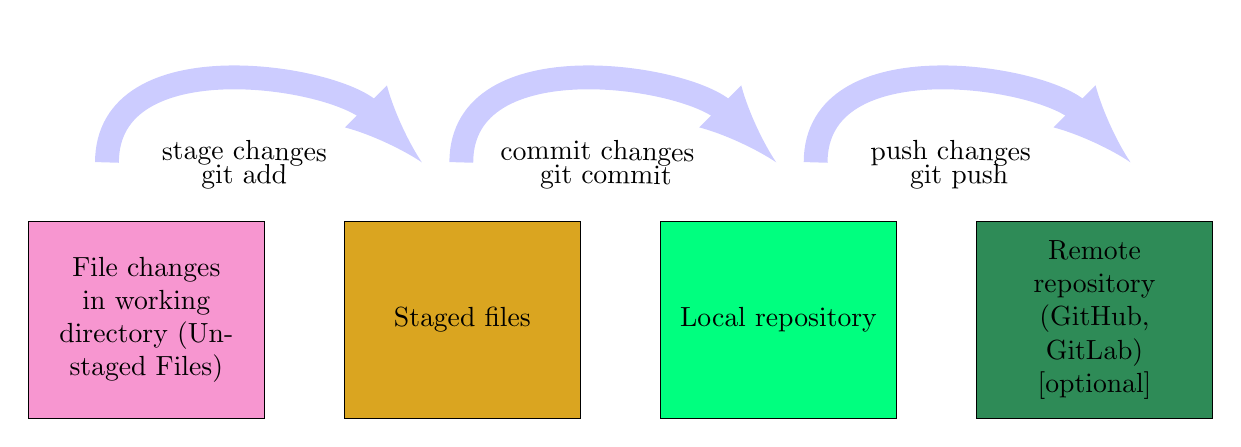
\begin{tikzpicture}[mypostaction/.style 2 args={decoration={text align={left indent=#1}, text along path, text={#2}},decorate}]
\node[draw,
      fill=Rhodamine!50,
      minimum width=3cm,
      minimum height=2.5cm,
      text width=2.5cm,
      text centered
     ]
	 (unstaged) at (0,0) {File changes in working directory (Unstaged Files)};
\node [draw,
       fill=Goldenrod,
	   minimum width=3cm,
	   minimum height=2.5cm,
	   text width=2.5cm,
	   text centered,
	   right=1cm of unstaged
	  ]
	  (staged) {Staged files};	 
\node [draw,
	   fill=SpringGreen, 
	   minimum width=3cm, 
	   minimum height=2.5cm,
	   text width=2.5cm,
	   text centered,
	   right=1cm of staged
	  ]
	  (local) {Local repository};	 
\node [draw,
       fill=SeaGreen, 
	   minimum width=3cm, 
	   minimum height=2.5cm,
	   text width=2.5cm,
	   text centered,
	   right=1cm of local
	  ]
	  (remote) {Remote repository (GitHub, GitLab) [optional]};
	 
% Arrows with text label
\coordinate (unstageRoot) at (-0.5,2); \coordinate (stageRoot) at (3.5,2);
	\draw[-latex, blue!20!white, line width=2ex]  (unstageRoot) to[in=135,out=90] (stageRoot);
	\path [postaction={mypostaction={0.7cm}{stage changes}},postaction={mypostaction={1.2cm}{git add},/pgf/decoration/raise=-3mm}](unstageRoot) to [in=180,out=3] (stageRoot);
\coordinate (stageRoot) at (4,2); \coordinate (localRoot) at (8,2);
	\draw[-latex, blue!20!white, line width=2ex]  (stageRoot) to[in=135,out=90] (localRoot);
	\path [postaction={mypostaction={0.5cm}{commit changes}},postaction={mypostaction={1cm}{git commit},/pgf/decoration/raise=-3mm}](stageRoot) to [in=180,out=3] (localRoot);
\coordinate (localRoot) at (8.5,2); \coordinate (remoteRoot) at (12.5,2);
	\draw[-latex, blue!20!white, line width=2ex]  (localRoot) to[in=135,out=90] (remoteRoot);
	\path [postaction={mypostaction={0.7cm}{push changes}},postaction={mypostaction={1.2cm}{git push},/pgf/decoration/raise=-3mm}](localRoot) to [in=180,out=3] (remoteRoot);

\end{tikzpicture}

You do your work in your \textbf{working directory}.
On the \textbf{stage} you collect all the changes that you want to save.
This is very powerful because sometimes it is just individual lines of code or text that you want to keep track of and not the whole file.
Once you've tracked all the changes that you want to combine, it is time to collect these changes into a \textbf{commit}.
A commit is a permanent snapshot of the files that git tracks stored in the {.git} directory.
It is associated with a unique identifier (hash).
In other words, a commit is like a snapshot in time; you can always revert back to this and see what changes were made compared to any other commit.
On your local repository (i.e.\ on your local machine) you now have a nice versioned history.
However, if you want to collaborate with others or sync your repository to a specialized cloud provider you need to push these changes to a so-called remote repository,
  typically on GitHub, GitLab, but any folder that you can access via remotely might serve as a remote repository.

\item
Click on the file and select \texttt{Stage File} or add each line by clicking on the plus or minus signs left to each line.
Once you are happy with the file, click on the X to close the file-comparison window.
We now don't see any unstaged files and can proceed to write a commit message and then click on the big green button.

\item
A \emph{good commit} typically does one discrete task or change only.
For example, you added a variable to the regression specification in the code, in the output and in the report.
Or you changed the name of a variable and treat it properly across multiple scripts.
This enables you to make meaningful commit messages like \emph{Add wage rigidities to the model} or \emph{Fix bug in the simulation routine}
  and you thus end up with a well organized repository.
This workflow needs some practice and everyone is slightly different with regards to this.
Nevertheless, try to combine changes to certain meaningful smaller tasks and provide good commit messages.
In my experience, having ten tiny commits is always preferable to one large commit.
Your future self and collaborators will thank you!

The question to what you should include in your commits, is also a matter of choice and preference.
Definitely your script files of codes, latex and text files.
Data is also sometimes given as csv files which are basically just text files.
Binary files (like Excel sheets, Word documents, Power Point slides) are a bit tricky to handle,
  as you can't see the differences between versions in git.
It depends on the specific needs whether one should commit these files as well (e.g.\ for Excel files with data this obviously makes sense),but I usually don't do this.
Note that GitHub doesn't allow files larger than 100 MB or projects with total size larger than 1 {GB}.
There is also a way to deal with large binary files called \texttt{Git Large File Storage (LFS)}.

\item
Right click on the initial commit and select \emph{Reset main to this commit {-} Soft}.
Click on the file in the staged files section and remove the last line from the stage.
Re-commit your stage by providing a meaningful commit message and hitting the green button.
Click on Stash to put the remaining changes into the stash.

\item
Simply click on Push and add the remote.
On the left Panel click on REMOTE to see the current remote (usually named origin).
Note that you can add several remotes (say from different people) and compare the commits.
Remotes are also a nice backup of your codes.

\item
Branches are arguably the most powerful part of \emph{git}.
By default you have a \textbf{main} branch,
  but what if you want to do some experiments, re-write an estimation function from scratch, work on a new feature, etc?
You could copy the whole folder and start working there or you use git and create a branch and make the changes there.
You can switch between branches, make commits to any branch, move them around, etc.
If your experiment doesn't work out, simply delete the branch.
If your experiments work out, commit them and merge them into the main branch.
Sometimes there will be conflicts which one needs to sort out,
  but using GUI tools like GitKraken makes this very easy
  as you have a pretty side-by-side comparison of changes.
Branches are arguably the most powerful part of \emph{git} especially for our purposes
  as research is a highly nonlinear process, and this way of doing version control is much more similar to how we actually work
  than the very linear way that other cloud storage providers do version control.
Branches are also extremely powerful for collaboration
  as different people can work on the same thing at the same time.

Select a so-called parent commit, where you want to create a new branch.
Note that this doesn't have to be the latest commit.
Click on the button \emph{Branch} and name it according to the exercise.
On the left panel, click on LOCAL to see an overview of all your branches.

\item
Create, copy and paste the three files into your repository.
Check for pasting errors and then \emph{Stage all changes} and commit them.

\item
Run the commands and solve any errors you might get from latex.

\item
Follow the instructions in the exercise.
Note that there is a difference between \enquote{Ignore} and \enquote{Ignore and Stop Tracking}.
\enquote{Ignore} simply adds the file{(type)} to the \texttt{.gitignore} file so that new files with that name/type/whatever are not tracked.
To \enquote{Ignore and Stop Tracking} means to remove the file{(s)} from git version control:
  they will no longer be in the repo (as of the commit that performs the \enquote{stop tracking}).
Basically, use \enquote{Ignore and Stop Tracking} if the file{(s)} you are ignoring never should have been in the repo in the first place.

\item
Make sure you are on the correct branch \emph{latex-exam-template} and push this branch to GitHub.
Either right click on the commit or go to the left panel, click on PULL REQUESTS and on the green plus sign that appears.
Select the \emph{latex-exam-template} as the FROM REPO branch and \emph{main} as the TO REPO branch.
Enter a Title and Description and click on the green button.
Have a look in GitHub ar the pull request.
As there are no conflicts merge it and go back to GitKraken to see what happens in your repository.
You might need to \enquote{fetch origin} by right clicking on the origin remote.

\item
Double click on your local main branch and then click on pull,
  which fast forwards your repo to the merged changes.
Then click on Pop to get the WIP codes which were stored on main.
Right click on the README.md file in the \emph{Unstaged Files} area and select \emph{Discard changes}.

\end{enumerate}
\fi
\newpage
\end{solution}\newpage
\printbibliography%
\newpage
\appendix
\section{Exam template files for \LaTeX}
\lstinputlisting[language=tex,frame=single,title=\lstname,breaklines=true,breakatwhitespace=false,basicstyle=\scriptsize\mlttfamily]{progs/latex/templateExamSolution.tex}
\lstinputlisting[language=tex,frame=single,title=\lstname,breaklines=false,breakatwhitespace=false,basicstyle=\scriptsize\mlttfamily]{progs/latex/templateExamBiblio.bib}
\lstinputlisting[style=Matlab-editor,basicstyle=\footnotesize\mlttfamily,title=\lstname]{progs/matlab/templateMatlabExample.m}


\Closesolutionfile{exercises_1_solution}
\ifDisplaySolutions%
\newpage
\section{Solutions}
\input{exercises_1_solution}
\fi
\end{document}